\documentclass[conference]{IEEEtran}
\IEEEoverridecommandlockouts
% The preceding line is only needed to identify funding in the first footnote. If that is unneeded, please comment it out.
\usepackage{cite}
\usepackage{amsmath,amssymb,amsfonts}
\usepackage{algorithmic}
\usepackage{graphicx}
\usepackage{textcomp}
\usepackage{xcolor}
\def\BibTeX{{\rm B\kern-.05em{\sc i\kern-.025em b}\kern-.08em
    T\kern-.1667em\lower.7ex\hbox{E}\kern-.125emX}}
\begin{document}

\title{Use environmental information and riding data to predict bicycle gear positions\\}

\author{\IEEEauthorblockN{1\textsuperscript{st} Cheng-Hsueh Ho}
\IEEEauthorblockA{\textit{Institute of Electrical Engineering College of Engineering} \\
\textit{National Chung Cheng University}\\
Chiayi 621, Taiwan \\
qack85112@gmail.com}
\and
\IEEEauthorblockN{2\textsuperscript{nd}Huei-Yung Lin, Ph.D.}
\IEEEauthorblockA{\textit{Institute of Electrical Engineering College of Engineering} \\
\textit{National Chung Cheng University}\\
Chiayi 621, Taiwan \\
 lin@ee.ccu.edu.tw}
}

\maketitle

\begin{abstract}
%本篇論文主要的目的是透過獲取騎乘者的生理訊息，與當下的環境資訊，選擇一個合適的檔位讓騎乘者可以順利地騎乘，不必顧慮檔位的切換問題。腳踏車平台我們使用先前建立的智慧自行車系統作為原型，該系統是一個可以即時的收集其逞者生理狀態與當下環境狀態的一個平台。並且選擇了幾種不同的決策方式對收集到的資料進行預測，透過收集到的感測器資訊對當下適合的檔位進行預測分析。由於有使用深度學習方面的方法，需要一定數量的資料用於進行訓練。我們使用先前建立的收集騎乘者生理資訊與環境資料的腳踏車系統，利用該系統收集騎乘者當下的多個感測器訊息。使用這些資料對我們所建立的機器學習方法進行訓練，最後透過一部分不包含在訓練資料內的資料對訓練後的結果進行測試。另外我們建立了一個網頁平台可以用於管理收集到的資料，該平台可以用於資料的上傳、查詢，還有簡單的分析結果可供查看。

The main purpose of this thesis is to obtain the physiological information of the rider, the current environmental information, and select a suitable gear so that the rider can ride smoothly without worrying about the problem of gear switching. We use the previously established smart bicycle system as a prototype to collect the physiological state of the rider and the current environmental state in real time. 
Several different decision-making methods are used with the collected sensor information to predict and analyze the current suitable gear. Due to the use of deep learning methods, a certain amount of data is required for training. We use the previously established bicycle system collect the physiological information and environmental data of the rider. After slightly adjusting the system, we use the system to collect the current multiple sensor information of the rider, as well as the current gear status. 
These data are used to train the machine learning method we have established, and finally methods are used for testing. In addition, we have established a web platform that can be used to manage the collected data. The platform can be used for data upload, query, and simple analysis for viewing.
\end{abstract}

%\begin{IEEEkeywords}
%\end{IEEEkeywords}

\section{Introduction}

%本篇論文的硬體部分是使用\cite{9026293}所建立的智慧自行車系統作為原型，加以調整後進行使用，該系統是一個可以即時的收集騎乘者生理狀態與當下環境狀態的一個平台，當時的系統也有對收集到的資料進行分析預測，但是因為著重在平台的建立，所以僅使用隨機森林的方式進行檔位的預測。

The hardware part of this paper is to use the smart bicycle system established by \cite{9026293} as a prototype, and adjust it for use. The system is a platform that can collect the physiological state of the rider and the current environmental state in real time. The system at that time also analyzed and predicted the collected data, but because it focused on the establishment of the platform, it only used the random forest method to predict the gear.

%近年來基於機器學習做為決策手段的方法越來越多，可是在腳踏車的領域多數的資料集僅包含了起點終點還有對應的時間這些訊息，如果只有這些訊息顯然對我們的檔位預測的訓練並沒有太大的有效性。所以我們自己收集一個資料集，該資料集包含了騎乘者的生理資訊與當下的環境資訊，與當下的檔位資訊，以利於我們使用機器學習的方法進行訓練。
In recent years, there have been more and more methods based on machine learning as a means of decision-making, but in the field of bicycles, most data sets only contain information such as the starting point and ending point and the corresponding time. If only these information are obviously predicting our gear Training is not very effective. So we collect a data set ourselves, which contains the physiological information of the rider, the current environment information, and the current gear information, so that we can use machine learning methods for training.

\begin{figure*}[h]
		\centering
		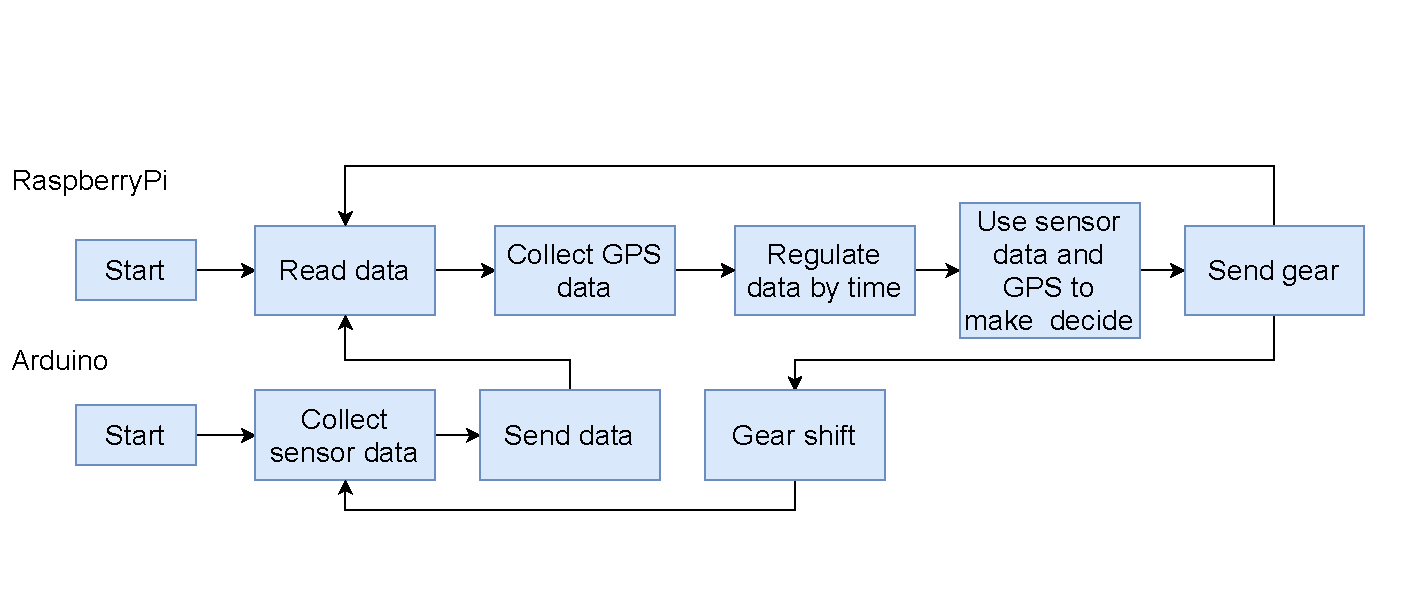
\includegraphics[width=\textwidth]{Image/simple_flow.pdf}
		\caption{Simple~flow~chart}
		\label{simple_Chart}
\end{figure*}
%圖\ref{simple_Chart}是基於\cite{9026293}的系統流程圖。系統分成兩個部分RaspberryPi和Arduino的部分，Arduino主要是作為收集資料與控制檔位的平台，在收集完資料後透過I2C傳遞給RaspberryPi，RaspberryPi再進行GPS的資料(位置與速度)收集，利用前面提到的決策方式對這些資訊決策出一個適合的檔位狀態再回傳給Arduino進行檔位的切換。

Figure \ref{simple_Chart} is a system flow chart based on \cite{9026293}. The system is divided into two parts, RaspberryPi and Arduino. Arduino is mainly used as a platform for collecting data and controlling gears. After collecting the data, it is transmitted to RaspberryPi through I2C. RaspberryPi then collects GPS data (position and speed). The mentioned decision-making method determines a suitable gear state based on the information and then sends it back to the Arduino to switch the gear.

\section{Related Work}
%在已經發表的文獻中對於腳踏車變速的決策方式有，透過腳踏的頻率並且加入模糊理論的方法\cite{1,2}，也有使用腳踏頻率與輪子轉速的關係來進行決策的\cite{tandon2011design}，還有以腳踏的壓力與車速來估計出道路坡度，再結合車輛載重的方式來決定出電動車適合功率的方法\cite{kai2017control}。和透過車速與曲柄的轉速來決定電動自行車升檔降檔的決策\cite{3}。這些的法都是透過車子的速度，曲柄轉速等方式來估計出變換檔位的決策，或是馬達功率，但是這些方法都缺少對於騎乘者的生理資訊，與對於真實環境的坡度，和道路狀況的分析。

In the published literature, the decision-making methods of bicycle speed change are as follows: the frequency of pedaling and the method of adding fuzzy theory \, and the method of using the relationship between pedal frequency and wheel speed to make decisions, there is also a method to estimate the road gradient based on the pressure of the pedals and the speed of the vehicle, and then combine the load of the vehicle to determine the appropriate power of the electric vehicle\cite{kai2017control}. And through the speed of the vehicle and the rotation speed of the crank to determine the decision of the electric bicycle to upshift and downshift. These methods use the speed of the car, crank speed and other methods to estimate the decision to change gears, or the motor power, but these methods lack physiological information for the rider, and for the slope of the real environment, and the road. Analysis of the situation.

%在\cite{coleman1920correlation}\cite{blain2009time}這兩篇論文中得知在騎乘者處於心情平靜的狀態下，心律的速度會與運動的頻率有直接的關聯。而在\cite{bertucci2005effects}提到了雖然不少的競技自行車手在爬坡的環境中會以較低的踩踏頻率騎乘，但是研究\cite{patterson1990bicycle}顯示上坡時較高的踩踏節奏可以提高騎乘的性能表現。並且本文使用\cite{kalman1960new}提供的IMU結合卡爾曼濾波器的方式，來估計出車體的傾斜狀態並且濾除雜訊，藉此做為調整檔位的部分參考依據。

In the two papers \cite{coleman1920correlation}\cite{blain2009time}, it is known that when the rider is in a calm state, the speed of the heart rhythm is directly related to the frequency of exercise.
In \cite{bertucci2005effects} it is mentioned that although many competitive cyclists ride at a lower pedaling frequency in a climbing environment, the research \cite{patterson1990bicycle} shows that a higher pedaling rhythm can be improved when going uphill. Riding performance. And this article uses the IMU provided by \cite{kalman1960new} combined with the Kalman filter to estimate the tilt state of the car body and filter out the noise, which is used as a part of the reference basis for adjusting the gear.


%而在檔位決策的部分我們分別使用了Random Forests\cite{breiman2001random}、Deep Forest\cite{zhou2017deep}、XGBoost\cite{chen2016xgboost}、LightGBM\cite{ke2017lightgbm}、CATBoost\cite{dorogush2018catboost}，並且因為最近使用神經網路來進行決策的方法還蠻熱門的，甚至\cite{sun2019supertml}還特地將表格數據建成一張圖來實現表格數據的捲機神經網路，所以我們也有使用神經網路的方法來進行檔位的決策。

In the part of gear decision we used Random Forests\cite{breiman2001random}, Deep Forest\cite{zhou2017deep}, XGBoost\cite{chen2016xgboost}, LightGBM\cite{ke2017lightgbm}, CATBoost\cite{dorogush2018catboost}, and because Recently, the method of using neural networks for decision-making is quite popular, and even \cite{sun2019supertml} specially builds the table data into a picture to realize the neural network of the table data, so we also have the method of using the neural network To make gear decisions.

%利用上述這些方法對對收集的IMU、心律、腳踏壓力、溫度資訊、GPS等資訊，透過使用預先收集的資訊作為輸入而手動變換的檔位做為ground truth訓練模型，用於即時對偵測到生理與環境資訊進行檔位的決策。

Using the above methods to collect information such as IMU, heart rhythm, foot pressure, temperature information, GPS, etc., by using pre-collected information as input and manually changing gears as ground truth training models for real-time detection Use physiological and environmental information to make gear decisions.

\section{Hardware system}
%這個章節主要會先回顧使用的硬體平台\cite{9026293}的架構，並且對於調整增加的部分進行說明。接著會對這個系統的運作流程除了檔位預測的部分進行介紹，包含了在收集訓練資料時、實際進行測試時，分別如何對資料進行收集。

This section will first review the architecture of the hardware platform \cite{9026293} used, and explain the adjustments and additions. Next, the operation process of this system will be introduced in addition to the part of gear prediction, including how to collect data when collecting training data and when actually testing.
\subsection{Hardware review}
%本小節對\cite{9026293}的系統，還有本篇論文中增加與調整的部分進行介紹與說明。圖\ref{bike}是該系統的整體圖片。圖\ref{bike}紅框5的部分是整個系統的核心，包含了Arduino與RaspberryPi都安裝在那個位置，並且RTC時間模組、GPS模組、IMU模組、電子變速系統的換檔的按鈕開關，也是安裝在該平面上，Arduino 作為主要的感測資訊收集還有馬達的控制，RaspberryPi則是作為資料分析的平台並且在必要時可以將資料上傳至資料庫。該系統的電子變速系統是透過馬達帶動的如圖\ref{bike}的紅框1所示，，圖\ref{bike}的紅框4是該系統的電力來源。接著圖\ref{bike}的紅框2是該系統的壓力感測器。圖\ref{bike}的紅框7的部分，這部分是一個手指脈搏感測器。圖\ref{bike}的紅框6的部分則是霍爾效應感測器，利用該感測器搭配一固定在輪子內側的磁條來對騎乘速度進行估計。

This subsection introduces and explains the system of \cite{9026293}, as well as the additions and adjustments in this paper. Picture \ref{bike} is the overall picture of the system. Figure \ref{bike}The part in red box 5 is the core of the whole system, including the Arduino and RaspberryPi are installed in that position, and the RTC time module, GPS module, IMU module, and electronic transmission system shift buttons The switch is also installed on this plane, and the Arduino serves as the main sensing information collection and motor control. RaspberryPi is used as a data analysis platform and can upload data to the database when necessary. The electronic transmission system of this system is driven by a motor as shown in the red box 1 of \ref{bike}, and the red box 4 of \ref{bike} is the power source of the system. Next, the red box 2 of \ref{bike} is the pressure sensor of the system. Figure \ref{bike}Red box 7, this part is a finger pulse sensor. Figure \ref{bike} The red frame 6 is a Hall effect sensor, which is used with a magnetic strip fixed on the inner side of the wheel to estimate the riding speed.


\begin{figure}[htbp!]
	\centering
	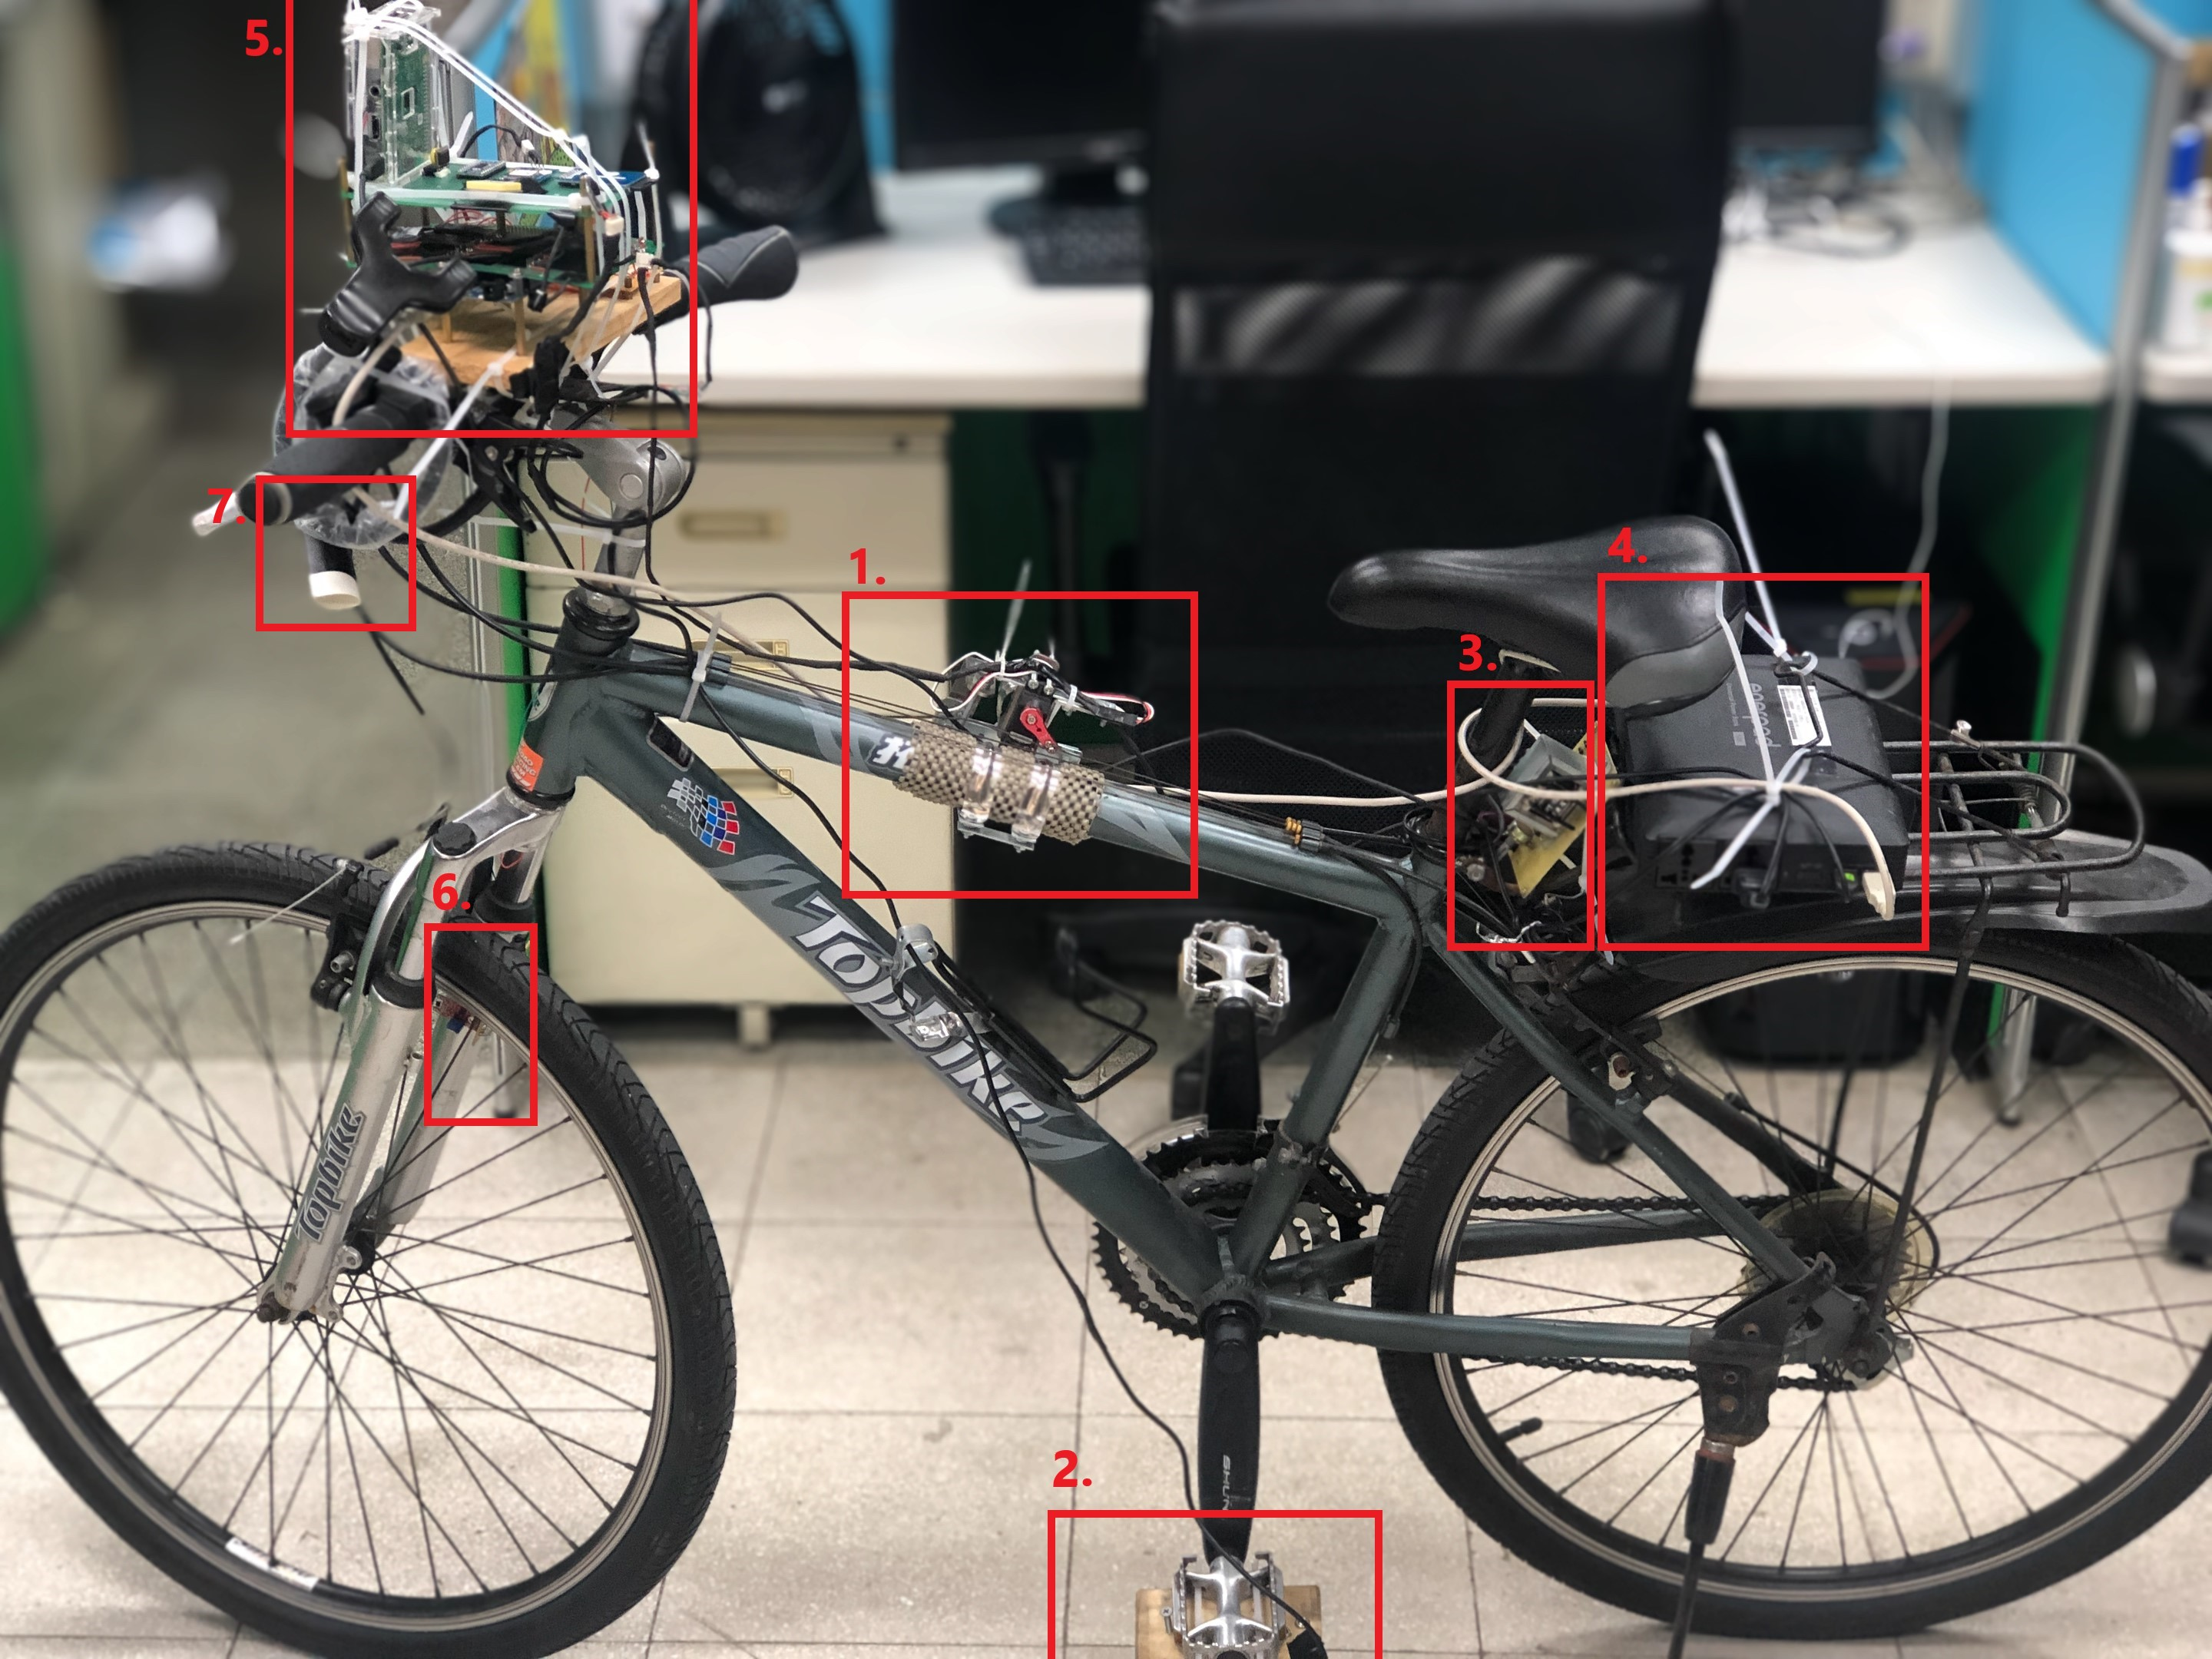
\includegraphics[width=0.4\textwidth]{Image/bike_1.jpg}
	\caption{Physical~image~of~bicycle}
	\label{bike}
\end{figure}

\subsection{Hardware adjustment}
%首先我們認為溫度訊息也會一定程度的影響騎乘者的騎乘狀態，所以我們在該系統中加入了一個溫度感測器模組用於環境溫度的檢測。本篇論文選用的是Heat-Sensitive Temperature Switch Sensor Module w這個NTC的熱敏電阻溫度感測器。

First of all, we believe that the temperature information will also affect the riding state of the rider, so we added a temperature sensor module to the system to detect the ambient temperature. In this paper, the NTC thermistor temperature sensor, Heat-Sensitive Temperature Switch Sensor Module w is selected.

%在速度感測的部分，原先是利用霍爾效應感測器搭配一固定在輪子內側的磁鐵實現的。但因為使用霍爾效應感測器來偵測速度的話，需要密集的在輪子旋轉時進行採樣，在此期間無法分心去對其他感測器進行採樣，又因為Arduino屬於單核心的平台，所以無法使用multi-thread的方式獨立一個核心進行採樣，導致占用整個Arduion太多計算量，使整體感測器的採樣頻率降低，並且出現空窗期，讓整個系統的採樣率不構平滑，進而導致收集的資料可信度不高。作為替代方案在收集訓練資料時速度資訊的部分使用GNSS同時會提供的速度資訊作為替代。

The speed sensing part was originally realized by using a Hall-effect sensor with a magnet fixed on the inner side of the wheel. However, Hall effect sensors need to be intensively sampled when the wheel is rotating. During this period, they cannot be distracted to sample other sensors, and the Arduino is a single-core platform, so it is impossible to use a multi-thread approach to stand alone. The core performs sampling, which takes up too much calculation of the entire Arduion, reduces the sampling frequency of the overall sensor, and a window period occurs, which makes the sampling rate of the entire system unsmooth, resulting in low credibility of the collected data. As an alternative, the speed information provided by GNSS is used as an alternative when collecting training data.

\subsection{System process and architecture}
%圖\ref{train}是本系統在收集資料時的流程圖，因為不需要利用感測器資料進行檔位判斷，所以就沒有了將Arduino資料傳遞到樹梅派的部分，檔位切換的部分由按鈕代替，並將這個檔位訊息作為ground turth，並且也將重複確認網路狀態的部分去除。另外感測器採樣的部分選擇使用protothread對每個感測器的採樣時間進行排程，這樣同時可以較輕易的控制採樣頻率，也可以將IMU的排程頻率提高來替代高頻率的中斷。

Figure \ref{train} is the flow chart of the system when collecting data, because there is no need to use sensor data for gear judgment, so there is no part of transmitting Arduino data to RaspberryPi, and the part of switching gears. Replace it with a button, and use this gear message as the ground turth, and also remove the part that repeats the confirmation of the network status. In addition, the sensor sampling part chooses to use protothread to schedule the sampling time of each sensor, so that the sampling frequency can be controlled more easily, and the scheduling frequency of the IMU can also be increased to replace high-frequency interrupts.

%圖\ref{train}的流程一開始Arduino會先對感測器、馬達進行初始化設定，接著設定用於換檔的中斷副程式，然後使用protothread設定每個感測器的採樣順序與頻率，接著就藉由設定好的排程讓系統一直運作下去，期間當中斷被觸發時就根據按鈕決定升降。
%RaspberryPi的部分因為不用對Arduino的sensor data進行資料分析，所以主要的工作只有收集GPS的資訊，包含速度與位置資訊，會將GPS資訊讓RaspberryPi處理主要是因為GPS的連接需要時間而RaspberryPi比Arduino穩定不少，且可以透過SSH等方式進行無線控制。

Figure \ref{train} At the beginning of the process, Arduino will first initialize the sensor and motor, set the interrupt subroutine for shifting, use protothread to set the sampling sequence and frequency of each sensor, and then borrow The set schedule keeps the system running, and during the period when the interrupt is triggered, it decides to increase or decrease according to the button.
RaspberryPi does not need to analyze the sensor data of Arduino, so the main work is only to collect GPS information, including speed and location information. The GPS information will be processed by RaspberryPi mainly because GPS connection takes time and RaspberryPi is more stable than Arduino Many, and can be controlled wirelessly through SSH and other methods.

\begin{figure*}[h]
	\centering
	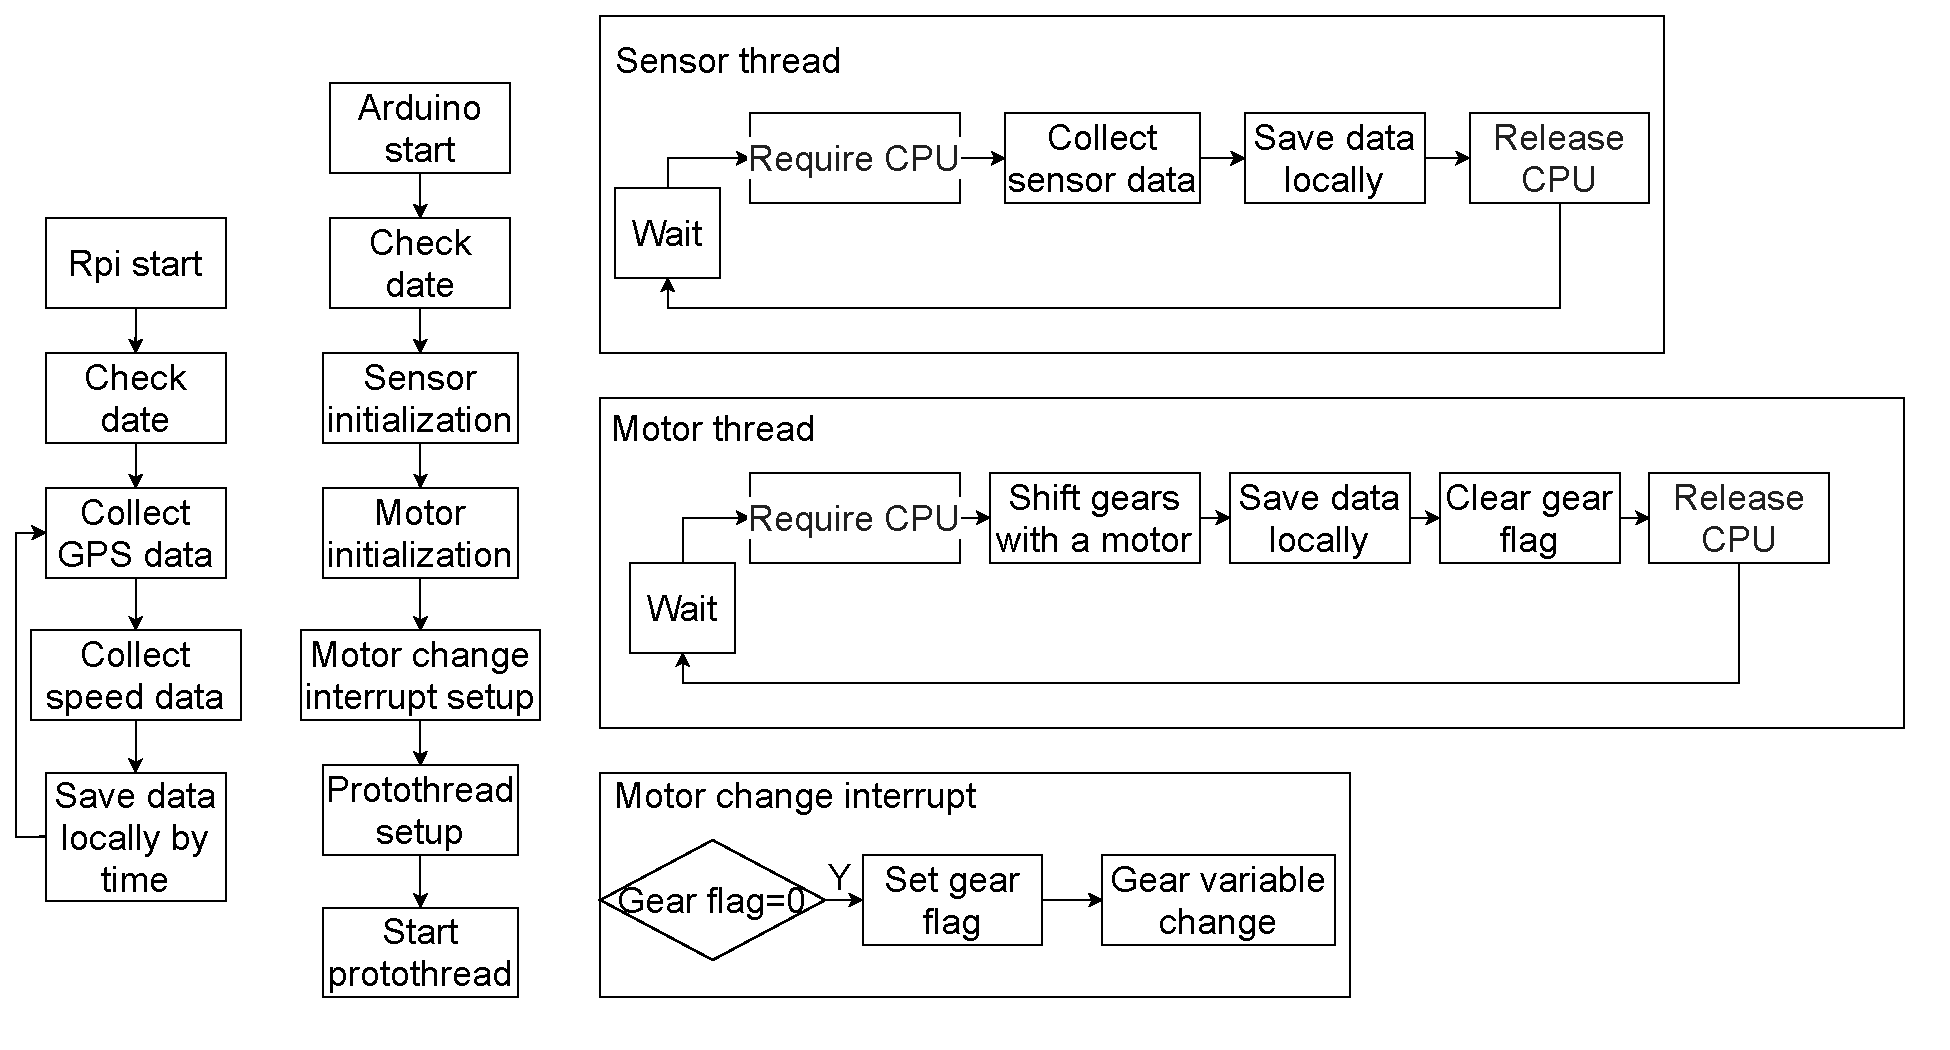
\includegraphics[width=1\textwidth]{Image/train_v2.pdf}
	\caption{Flow~chart~of~collecting~training~data}
	\label{train}
\end{figure*}

%測試階段的流程因為測試階段需要在騎乘時根據sensor data、GPS(包含速度與位置資訊)，還有圖資這些訊息來進行及時的檔位判斷。所以這部分與圖\ref{train}主要的差別就是會將Arduino的資料透過I2C傳遞給RaspberryPi，還有Arduino原本使用按鈕進行手動換檔的部分，替換成在Arduino將感測器資料傳送出去後等待RaspberryPi的檔位判斷的回傳，再進行檔位的切換。

The process of the test phase is because the test phase needs to use sensor data, GPS (including speed and location information), and map data to make timely gear judgments during riding. So the main difference between this part and the picture \ref{train} is that the Arduino data is transmitted to RaspberryPi through I2C, and the part where Arduino originally used buttons to manually shift gears is replaced by waiting for the RaspberryPi to determine the gear position, and then start the gear. Bit switching.

\section{Gear analysis system and web page construction}
%本章節首先會對本篇論文所使用的檔位預測方法進行介紹與說明，檔位預測的方法我們使用了包含Random Forests、Deep Forest、XGBoost、LightGBM、CATBoost，還有神經網路的方式進行決策。接著會對我們所建立的雲端資料庫系統還有網站的功能進行說明與介紹。

This section first introduces and explains the gear prediction method used in this paper. The gear prediction method we use includes Random Forests, Deep Forest, XGBoost, LightGBM, CATBoost, and neural networks to make decisions. Then we will explain and introduce the functions of the cloud database system and the website that we have built.

\subsection{Data analysis and gear forecast}
%檔位預測的方式我們選擇了包含Deep Forest、XGBoost、LightGBM、CATBoost、Random Forests，還有神經網路這幾種種方法分別進行測試。

For the method of gear prediction, we chose to test several methods including Deep Forest, XGBoost, LightGBM, CATBoost, Random Forests, and neural networks.

%輸入的特徵資訊包含了腳踏壓力、心律、IMU、環境溫度、GPS、移動速度，以上為一些基礎的訊息，另外加入地圖資訊，與前一個時間點的檔位，使用這兩種資訊結合基礎的感測器資訊一起用於檔位的預測。加入前次檔位訊息是因為只使用即時的資訊對檔位進行決策會有著資料處於兩個檔位的中間值，導致該時間段內檔位會頻繁的變動，這種變換檔位的方式並不符合大眾的騎乘習慣。因此我們將前次的檔位加入判斷，使其學習到如何根據前次檔位與感測器資料進行檔位的切換，同時學到檔位變換並不會短時間內頻繁的發生。

The input feature information includes pedal pressure, heart rate, IMU, ambient temperature, GPS, and moving speed. The above is some basic information. In addition, map information and past gear are added. Use these two information to combine basic sensor information. Used together for gear prediction. The past gear information is added because only real-time information is used to make a gear decision. The data will be in the middle of the two gears, resulting in frequent changes in the gear during this time period. This way of shifting gears does not conform to the riding habits of the public. Therefore, we add past gear to the judgment, so that it can learn how to switch gears based on the previous gear and sensor data, and learn that gear changes will not happen frequently in a short time.

%XGBoost、LightGBM、CATBoost、Deep Forest、Random Forests直接對我們的資料進行預測時準確度不低但是有著高頻率的檔位變動，若直接加入past gear的訊息會對檔位訊息產生過度的依賴。因此我們使用兩階段預測的方式來進行訓練，如圖\ref{XGB}所示一開始會先使用沒有past gear的輸入資訊進行一次預測，出來的結果會有著高頻率的變動，若用該資訊作為past gear就會因為不是真正的ground turth，所以不會有過度依賴的問題，所以我們就將預測出來的檔位依序作為past gear的訊息加入前一個時間點的輸入特徵中，以進行下一次的訓練，接著在二階段的訓練中就使用包含著past gear的訊息來進行訓練，並重複第二階段一定次數後停止，得到最終的結果。這樣就可以在考慮past gear的同時又不會對past gear 產生過度的依賴。

When XGBoost, LightGBM, CATBoost, Deep Forest, Random Forests directly predict our data, the accuracy is not low, but there are high-frequency gear changes. If the information of past gear is directly added, it will be excessively dependent on the gear information. Therefore, we use a two-stage prediction method for training. As shown in the figure \ref{XGB}, we will first use the input information without past gear to make a prediction, and the results will have high frequency changes. If this information is used As a past gear, because it is not a real ground turth, there will be no over-reliance. Therefore, we will add the predicted gears as the information of the past gear to the input characteristics at the previous time point in order to proceed. Training once, then use the information containing the past gear to train in the second stage of training, repeat the second stage a certain number of times and then stop to get the final result. In this way, the past gear can be considered while not being overly dependent on the past gear.

\begin{figure*}[htbp]
	\centering
	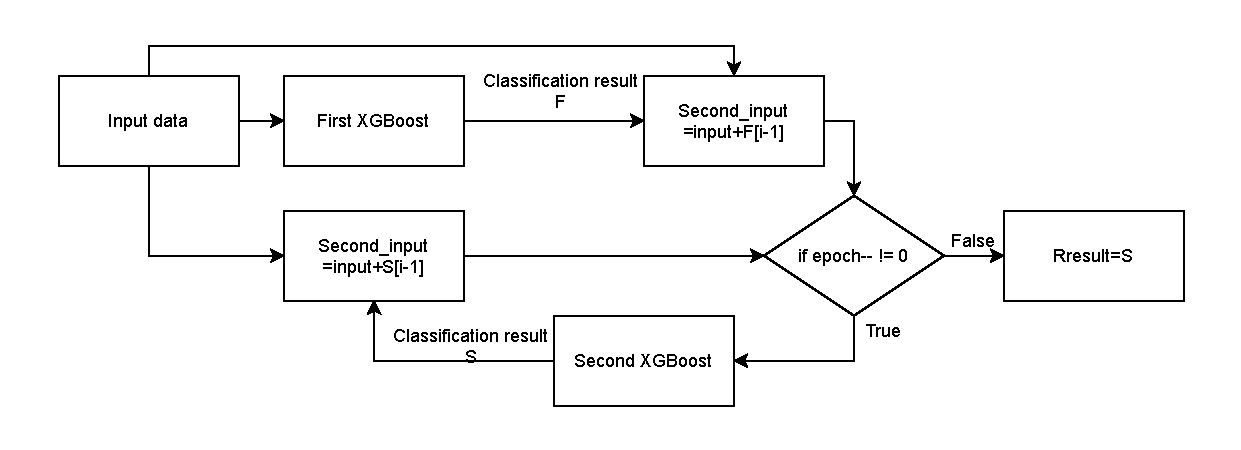
\includegraphics[width=0.8\textwidth]{Image/XGB_v2.pdf}
	\caption{Two-stage training: the first stage of training does not consider the past gear, the second stage uses the first-stage prediction result as the past gear information for training, and repeats epoch times}
	\label{XGB}
\end{figure*}
%在神經網路的部分我們選擇的預測方法主要是參考Artificial Neural Network\cite{wang2003artificial}，並另外參考ResNet\cite{he2016deep}與UNet\cite{he2016deep}的部分模型架構的方法。

In the part of the neural network, the prediction method we choose is mainly to refer to the Artificial Neural Network\cite{wang2003artificial}, and also to refer to the part of the model architecture of ResNet\cite{he2016deep} and UNet\cite{he2016deep}.

%另外我們加入了圖資的訊息對一些人造的場景資訊一起進行分析，人造的場景中經常會有一些明明坡度沒有明顯的變化，生理上也沒有明顯的改變，可是確實需要換檔的狀況，像是紅綠燈、路口之類的像是這些狀況利用圖資的訊息提前進行判斷，就可以有效的使騎乘者有更好的騎乘體驗。

In addition, we have added information from the map to analyze some artificial scene information. In artificial scenes, there are often some obvious slopes that have no obvious changes, and there are no obvious changes in physiology. However, it is indeed necessary to change gears, such as It is the traffic lights, intersections, etc., such as these situations, using the information of the map to make a judgment in advance. It can effectively enable riders to have a better riding experience.


\subsection{Cloud building and web page hosting}
%網頁的建置在\cite{9026293}架設的網頁的基礎上進行完善，資料庫使用MySQL平台，網頁的模板為HTML5 UP所提供\footnote{HTML5 UP網頁模板license : https://html5up.net/license}，主要的功能有管理者的登入、騎乘資訊的查詢、資料登錄、資料分析這幾個部分，且管理者可以查詢多個騎乘者的狀況。

The web page is built on the basis of the web page set up by \cite{9026293}. The database uses the MySQL platform. The web page template is provided by HTML5 UP. \footnote{HTML5 UP web page template license: https://html5up.net/ license}, the main functions include administrator login, riding information query, data registration, data analysis, and the administrator can query the status of multiple riders.

%架構如圖\ref{webflow}所示，主要分為登入前與登入後兩個部分，登入前僅可察看首頁資訊，其他相關功能需要進行登入的動作後才可瀏覽操作，例如資料上傳、資料查詢、檔位分析等功能。

The structure is shown in Figure \ref{webflow}, which is mainly divided into two parts before login and after login. Before login, only the homepage information can be viewed. Other related functions need to be logged in before browsing operations, such as data upload and data Query, gear analysis and other functions.

\begin{figure*}[htbp]
	\centering
	
\includegraphics[width=1\textwidth]{Image/web/web_v2.pdf}
	\caption{Web page structure diagram, data query and upload can only be performed after login, and only login and registration related operations can be performed before login}
	\label{webflow}
\end{figure*}

\section{data collection}
%在資料集的部分大致上可以分為校內與校外兩個部分，校內的資料因為地形屬於較為規範的狀態，所以收集時會有一個固定規劃好的路線進行騎乘。校外因為較為開放所以騎乘時雖然還是會對路線有稍微規劃，但是並不會完全的依照事前規劃所行動，且騎乘習慣也與校內的狀態有些許的差異。

The dataset can be roughly divided into two parts: inside and outside the school. Because the information in the school is in a more standardized state, there will be a fixed and planned route for riding when collected. Because the outside of the school is relatively open, although there is still a slight plan for the route when riding, it will not completely follow the pre-planned action, and the riding habits are slightly different from the state of the school.

%圖\ref{school1}[a-e]為學校內主要收集資料的路線，並且因為是屬於較規範的路線，所以每個路線大致上都收集了約10,000筆資料，總計收集50,000筆資料用來訓練，並且每個路線都有包含上坡下坡、平地這些不同的路況，而有2個路線中有包含到重要的道路標記的位置。

Figure \ref{school1}[ae] is the main route for collecting data in the school, and because it is a more standardized route, roughly 10,000 data are collected for each route, and a total of 50,000 data are collected for training. And each route has different road conditions including uphill, downhill, and flat ground, and there are two routes that contain important road markings.
\begin{figure*}[htbp]
	\centering
	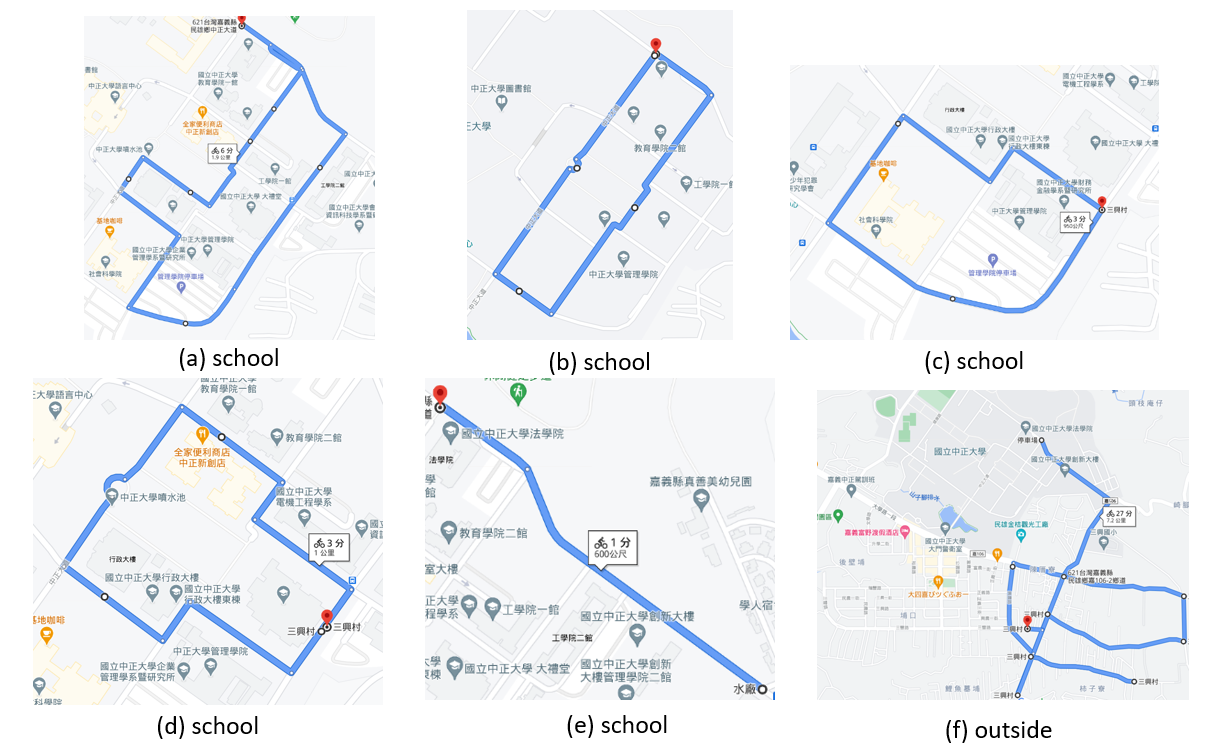
\includegraphics[width=0.8\textwidth]{Image/TrainPath.png}
	\caption{Training dataset}
	\label{school1}
\end{figure*}

%圖\ref{school1}[f]是我們收集的校外資料集所包含的所有路線的狀況，總資料量大約有50,000筆進行訓練。

The picture \ref{school1}[f] is the status of all the routes included in the data set outside the school we have collected. The total amount of data is about 50,000 for training.

\section{Experiment}
%在測試的部分我們會分成幾個章節對不同的方法分開進行測試。圖\ref{schooltest}是我們用來進行校內測試的資料集，其範圍涵蓋了許多訓練資料中出現的場景。

In the testing part, we will be divided into several chapters to test different methods separately. The picture \ref{schooltest} is the data set we use to conduct school tests, and its scope covers many scenes that appear in the training data.

A score evaluation formula \ref{score} suitable for our application situation is designed. The standard is set as the ratio of accuracy minus the variation score ~osc~ and the number of samples ~sa~. Because we don’t want the gear to switch too frequently, we set the change score to negative. The method is to use a sliding window with a size of ~sl~ to scan from the beginning to the end of the test data. When the gear is within 2 seconds ~G~ changes more than twice, accumulate the number of changes $\mu$ and divide by the number of samples. In addition, the accuracy is compared by the ground turth and the prediction result. When the two are the same, the count is counted and the overall ratio is calculated.
\begin{equation}
\begin{aligned}
Score= Accuracy - osc/sa\\
osc=\sum_{n=0}^{n= sa - sl}\left\{\begin{matrix}
0&\mu < 2\\ 
\mu&\mu\geq 2
\end{matrix}\right.\\
\mu=\sum_{m=n}^{m=n+sl-1}\left\{\begin{matrix}
 0&G[m]=G[m+1] \\
 1&G[m]\neq G[m+1] 
\end{matrix}\right.
\end{aligned}
\label{score}
\end{equation}
\subsection{Neural network}
%首先我們對使用神經網路的方法進行討論，這部分的測試資料有包含了重要標記的訊息，圖\ref{schooltest}[b]的紅色框部分就是經過該標記時，因為該標記而提早提升檔位，可以看到圖\ref{schooltest}[b]有預測到這件事情。

First, let’s discuss the method of using neural networks. This part of the test data contains information about important markers. The red box in the picture \ref{schooltest}[b] is when the marker is passed, it is promoted early because of the marker. For the gear, you can see that the picture \ref{schooltest}[b] predicted this.

\begin{figure*}[htbp]
	\centering
	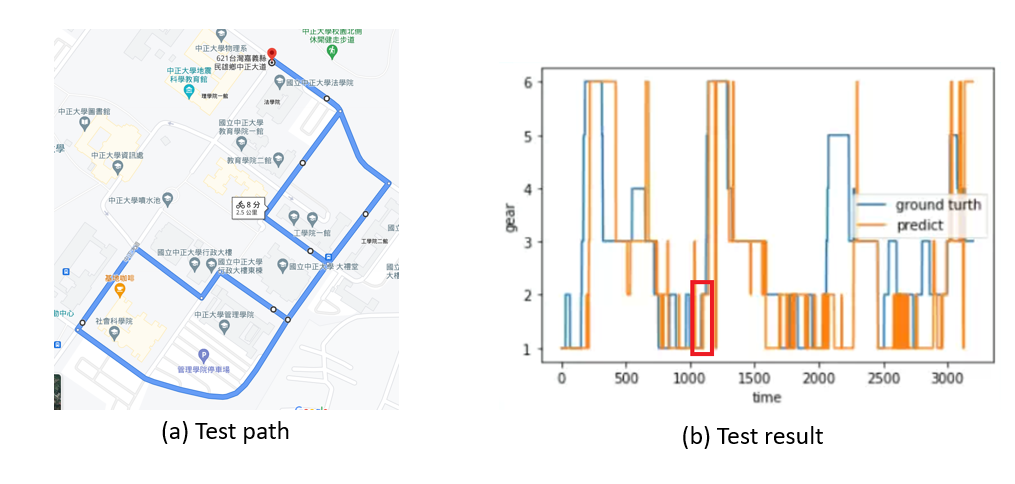
\includegraphics[width=0.8\textwidth]{Image/TestPath.png}
	\caption{School~test}
	\label{schooltest}
\end{figure*}




%為了確認加入past gear 對我們整個架構可以得到哪一些影響，所以有特別的比較同樣的架構下有考慮past gear和沒有考慮past gear各自的預測狀況，圖\ref{WithWithoutGearNN}的左圖是沒有考慮past gear的狀況，可以看到整個圖片中有許多很頻繁的震盪，而圖\ref{WithWithoutGearNN}的右圖則是有考慮past gear的狀況，可以明顯的看出相比不考慮past gear的左圖，那些高頻率震盪的部分基本上都沒有出現了，從這兩張圖中可以很明顯的看出，在網路中加入past gear進行判斷，可以更加符合人類的騎乘習慣，讓其不太會出現高頻率在兩個檔位中震盪的狀況。

In order to confirm the impact of adding past gear to our entire architecture, there is a special comparison between considering past gear and not considering past gear’s respective forecast conditions under the same architecture.The left picture of the picture \ref{WithWithoutGearNN} does not consider the condition of the past gear. It can be seen that there are many frequent oscillations in the whole picture, and the picture on the right of the picture \ref{WithWithoutGearNN} is the condition of the past gear. It is obvious that compared to the left picture without considering the past gear, those high-frequency oscillations have disappeared. From these two pictures, it is obvious that adding past gear to the network for judgment can be more in line with human riding habits. .

\begin{figure*}[htbp]
	\centering
	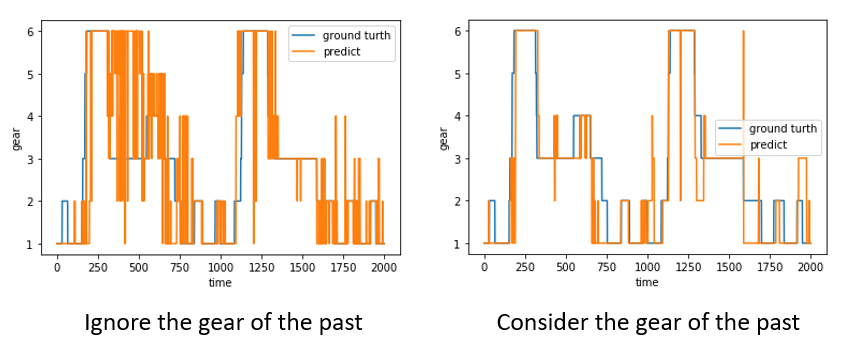
\includegraphics[width=0.8\textwidth]{Image/NNtest/WithWithoutGear0605.png}
	\caption{NN compares whether past gear is considered}
	\label{WithWithoutGearNN}
\end{figure*}

\subsection{Random Forests}
%我們使用\cite{9026293}論文中有使用到的Random Forests方法進行測試。圖\ref{WithWithoutGearRF}的左圖是使用原始的Random Forests的效果，可以看到整體輪廓與準確度都不差，但是整體而言檔位變換的頻率過高，這應該是因為沒有考慮past gear進行判斷的關係，因此圖\ref{WithWithoutGearRF}的右圖我們加入了past gear的訊息一起進行決策，可以看到整體的檔位變動頻率降低了不少。

We use the Random Forests method used in the \cite{9026293} paper for testing. The left image of the picture \ref{WithWithoutGearRF} is the effect of using the original Random Forests. It can be seen that the overall profile and accuracy are not bad, but the frequency of gear shifting is too high overall. This should be because the past gear is not considered The relationship of making judgments. Therefore, in the right picture of the picture \ref{WithWithoutGearRF}, we added the information of the past gear to make a decision. We can see that the overall gear change frequency has been reduced a lot.
\begin{figure*}[h]
	\centering
	
\includegraphics[width=0.8\textwidth]{Image/RF/withwithoutpastgear.png}
	\caption{RF compares whether past gear is considered}
	\label{WithWithoutGearRF}
\end{figure*}
\subsection{Deep Forest}
%使用DeepForest對我們的資料進行分析，圖\ref{WithWithoutGearDF} 的左圖為使用原始的DeepForest方法，不考慮前次檔位進行測試，可以看/到整體而言檔位的變動頻率過高並不符合人體的騎乘習慣，圖\ref{WithWithoutGearDF}的右圖加入了前次檔位的訊息，明顯的看到檔位變動頻率降低。

Use DeepForest to analyze our data. The left picture of the picture \ref{WithWithoutGearDF} uses the original DeepForest method and does not consider the previous gear for testing. It can be seen that the overall frequency of gear changes is too high. In line with the riding habits of the human body, the picture on the right of the picture \ref{WithWithoutGearDF} has added the information of the previous gear. It is obvious that the frequency of gear changes is reduced.
\begin{figure*}[h]
	\centering
	
\includegraphics[width=0.8\textwidth]{Image/DF/withwithoutpastgear.png}
	\caption{DF compares whether past gear is considered}
	\label{WithWithoutGearDF}
\end{figure*}

\subsection{XGBoost,LightGBM,CATBoost}
%最後我們使用XGBoost、LightGBM、CATBoost這三種方法分別對我們的資料集進行分析，圖\ref{WithWithoutGearXGB}的左圖是使用原始的XGBoost調整參數後的測試結果，可以看到XGBoost的方法本身就有著不確的準確度，且在整體的預測輪廓上也符合ground turth，但是在整個預測的過程中因為沒有考慮到past gear的訊息，所以整體的預測結果經常會有頻繁變動的狀況，為了改善這個狀況我們加入了第三中所提到的兩階段的訓練方式在訓練中加入了past gear的訊息，結果如圖\ref{WithWithoutGearXGB}的右圖所示，從圖中可以看到整體的穩定性提升了不少，幾乎沒有頻繁改變檔位的問題了，並且在準確度方面也與原本的XGBoost差距不大。圖\ref{WithWithoutGearLGBM} 圖\ref{WithWithoutGearCAT}的左圖同樣是不考慮前次檔位的LightGBM與CATBoost，兩個方法的準確度都有一定水準，但是檔位變動的頻率依然太高了，圖\ref{WithWithoutGearLGBM} 圖\ref{WithWithoutGearCAT}右圖為使用了兩階段訓練的方式加入了前次檔位後，整體的穩定度提升了許多。

Finally, we use XGBoost, LightGBM, CATBoost these three methods to analyze our data set, the left picture of the picture \ref{WithWithoutGearXGB} is the test result after using the original XGBoost to adjust the parameters, you can see that the XGBoost method itself has The accuracy is inaccurate, and the overall prediction profile is also in line with the ground turth. However, because the past gear information is not taken into account during the entire prediction process, the overall prediction results often change frequently. In order to improve this Situation We have added the two-stage training method mentioned in the third and added the message of past gear in the training. The result is shown in the right figure of \ref{WithWithoutGearXGB}, and the overall stability can be seen from the figure. It has improved a lot, there is almost no problem of frequently changing gears, and the accuracy is not much different from the original XGBoost. The left picture of \ref{WithWithoutGearLGBM} \ref{WithWithoutGearCAT} also shows the LightGBM and CATBoost without considering the previous gear. The accuracy of the two methods has a certain level, but the frequency of gear changes is still too high. Picture \ref{WithWithoutGearLGBM} \ref{WithWithoutGearCAT} The picture on the right shows the use of a two-stage training method after adding the previous gear, the overall stability has improved a lot.

\begin{figure*}[h]
	\centering
	
\includegraphics[width=0.8\textwidth]{Image/XGB/withwithoutpastgear.png}
	\caption{XGBoost~compares whether past gear is considered}
	\label{WithWithoutGearXGB}
\end{figure*}

\begin{figure*}[h]
	\centering
	
\includegraphics[width=0.8\textwidth]{Image/LGBM/withwithoutpastgear.png}
	\caption{LightGBM compares whether past gear is considered}
	\label{WithWithoutGearLGBM}
\end{figure*}

\begin{figure*}[h]
	\centering
	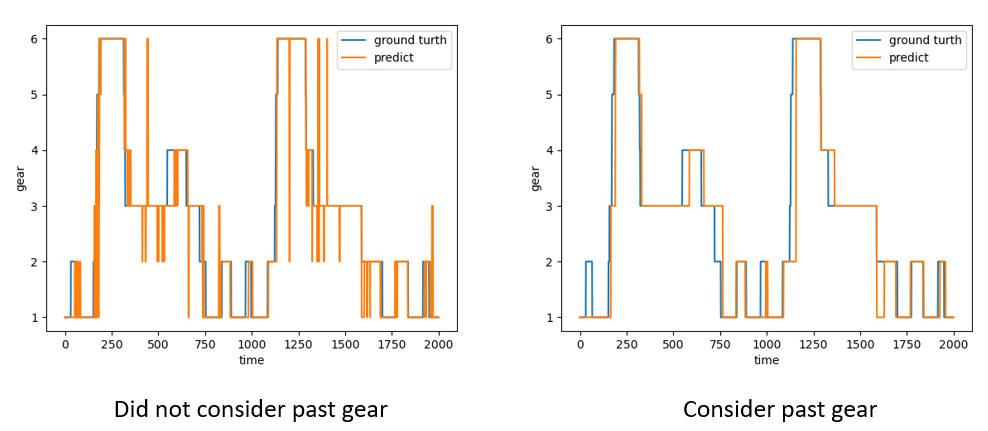
\includegraphics[width=0.8\textwidth]{Image/CAT/withwithoutpastgear.png}
	\caption{CATBoost compares whether past gear is considered}
	\label{WithWithoutGearCAT}
\end{figure*}


%由上述的實驗可以看出，在不加入past gear的狀況下雖然許多方法都可以在準確度方面有著不差的表現，但是總是會有檔位切換頻率過高的問題。因此我們使用了將past gear加入訓練的方法。分別使用稀釋與兩階段訓練的方式將past gear訊息加入訓練中。也可以看出使用兩階段方法的XGBoost、RF、LightGBM、CATBoost整體的變動頻率比起單純稀釋的NN、DF、RF又更低了一些。由此可知我們的兩階段的訓練方式是有效的。

It can be seen from the above experiments that although many methods can have good accuracy in terms of accuracy without adding past gear, there will always be a problem of too high gear switching frequency. So we used the method of adding past gear to training. Use the dilution or two-stage training method to add the past gear information to the training. It can also be seen that the overall fluctuation frequency of XGBoost, RF, LightGBM, and CATBoost using the two-stage method is lower than that of purely diluted NN, DF, and RF. This shows that our two-stage training method is effective.

\subsection{Discussion}
%由前面的實驗中可以得知在神經網路、Random Forests、Deep Forest、XGBoost、LightGBM、CATBoost這些方法中，神經網路的方法與預期一樣在表格數據集中的表現並不突出，剩下的幾種方法中在沒有考慮前次檔位情況下，幾個方法的準確度差距並不大，加入了前次檔位後XGBoost、LightGBM、CATBoost、Random Forests得益於可以利用迭代的方式多次訓練得到了比DeepForest更加讓人滿意的效果，其中又以XGBoos、CATBoost這兩種方法的效果最好。將所有資料加入一起訓練後，因為校內與校外資料騎乘習慣不同，效果都比單獨訓練時遜色了一些，或是僅有些微的提升。

%表\ref{ALLscore}表\ref{ALLscore2}為所有方法測試得出的準確度，橫軸是使用方法，縱軸是測試資料集，ALL代表使用校內與校外一同訓練。從表中可以看出XGBoost與CATBoost有著最高的得分，因此我們認為Boosting~Tree對於我們的資料集而言是很有效的。LightGBM雖然同樣是Boosting~Tree方法，但因為其輕量化的結構，並且LightGBM\cite{ke2017lightgbm}提到所測試的資料中與我們的資料差距很大，該論文中提到的資料集與特徵數量的大小比我們的大許多，因此我們認為該方法並不適合用於我們的資料。RandomForests仍然有不錯的準確度，但是略遜於XGBoost與CATBoost。而使用深度的隨機森林的DeepForest效果甚至比起RandomForests還差，因此我們認為我們的資料並不需要非常深的架構才能有效的預測。最後神經網路方法仍然並不適合用於我們這種表格形式的資料集，比起使用神經網路，樹狀結構的方法明顯可以產生較好的結果。

From the previous experiments, it can be known that among the neural network, Random Forests, Deep Forest, XGBoost, LightGBM, and CATBoost, the neural network method does not perform as expected in the table data set. The remaining few In this method, without considering the previous gear, the accuracy difference of the several methods is not large. After adding the previous gear, XGBoost, LightGBM, CATBoost, Random Forests benefit from the possibility of multiple training in an iterative manner. Obtained more satisfactory results than DeepForest, of which XGBoos, CATBoost these two methods have the best effect. After all the materials are added to the training, because the riding habits of the school and off-school materials are different, the effect is a little less than that of the training alone, or only slightly improved.

Table \ref{ALLscore} Table \ref{ALLscore2} is the accuracy of all methods tested, the horizontal axis is the method of use, the vertical axis is the test dataset, and ALL represents the use of school and outside training together. It can be seen from the table that XGBoost and CATBoost have the highest scores, so we think Boosting~Tree is very effective for our dataset. Although LightGBM is also the Boosting~Tree method, but because of its lightweight structure, and LightGBM\cite{ke2017lightgbm} mentioned that the data tested is far from our data, the dataset and the number of features mentioned in the paper The size of is much larger than ours, so we think this method is not suitable for our data. RandomForests still has good accuracy, but it is slightly inferior to XGBoost and CATBoost. The DeepForest effect using deep random forests is even worse than RandomForests, so we believe that our data does not require a very deep structure to effectively predict. Finally, the neural network method is still not suitable for our tabular dataset. Compared with the neural network, the tree structure method can obviously produce better results.

\begin{table}[h]
\centering 
\caption{Score summary table}\label{ALLscore}
\makebox{
\begin{tabular}{| c | c | c | c | c | c |}
\hline
 ~&XGB&CATBoost&LGBM&RF      \\ \hline 
school&0.785&0.808&0.732&0.727      \\ \hline
ALLschool&0.687&0.800&0.756&0.746     \\ \hline
outside&0.669&0.515&0.361&0.642      \\ \hline
ALLoutside&0.44&0.558&0.389&0.688    \\ \hline
\end{tabular}}
\end{table}

\begin{table}[h]
\centering 
\caption{Score summary table}\label{ALLscore2}
\makebox{
\begin{tabular}{| c | c | c | c | c | c |}
\hline
 ~&DF&NN    \\ \hline 
school&0.685&0.61      \\ \hline
ALLschool&0.65&0.586      \\ \hline
outside&0.456&0.478       \\ \hline
ALLoutside&0.396&0.481       \\ \hline
\end{tabular}}
\end{table}



\section{Conclusion}
%本篇論文基於\cite{9026293}建立的腳踏車騎乘者生理資訊、環境資訊收集，再加上電子變速系統，對其系統進行關於採樣頻率與系統穩定度方面的調整，並且利用調整後的平台對校內5條不同騎乘路線、與校外路線進行訓練資料的收集，另外收集了一筆校內、與校外資料作為我們的測試路線。使用數個機器學習、深度學習的方法對該資料集進行自車檔位的預測，使用的方法包含了神經網路、RandomForests、DeepForest、XGBoost、LightGBM、CATBoost這幾個，並且對這些方法進行調整優化，對所有的結果進行分析與討論，最後我們認為神經網路方法依舊無法有效的對表格類資料實行有效預測，其餘的方法中RandomForest、XGBoost、LightGBM、CATBoost得益於可以反覆進行學習因而得到了最令人滿意的效果，其中又以XGBoost與CATBoost的預測最為平順且符合測試資料的騎乘習慣。另外我們建立一個網頁平台，用於資料的儲存、查詢，與簡易的分析比較。供使用者了解自己的騎乘狀況，並確認該系統的預測與真實的狀況是否吻合。
This paper is based on the collection of physiological information and environmental information of bicycle riders established by \cite{9026293}, coupled with an electronic transmission system, to adjust the sampling frequency and system stability of the system, and use the adjusted platform We collected training data on 5 different riding routes in the school and off-campus routes, and collected a piece of on-campus and off-campus data as our test route. Use several machine learning and deep learning methods to predict the position of the vehicle on this data set. The methods used include neural networks, RandomForests, DeepForest, XGBoost, LightGBM, CATBoost, and these methods are adjusted. Optimize, analyze and discuss all the results. Finally, we believe that the neural network method is still unable to effectively predict the table data. Among the other methods, RandomForest, XGBoost, LightGBM, and CATBoost benefit from repeated learning. The most satisfactory results are achieved, among which the predictions of XGBoost and CATBoost are the smoothest and conform to the riding habits of the test data. In addition, we have established a web platform for data storage, query, and simple analysis and comparison. For users to understand their riding conditions, and to confirm whether the system’s predictions are consistent with the real conditions.
\bibliography{thesis}{}
\bibliographystyle{IEEEtran}


\end{document}
